\chapter{Further data analysis}

%TODO include maps of zones, and tables of population and empoyment values etc
%TODO sections and horizonal lines in appendicies
\begin{figure}[H]
\centering
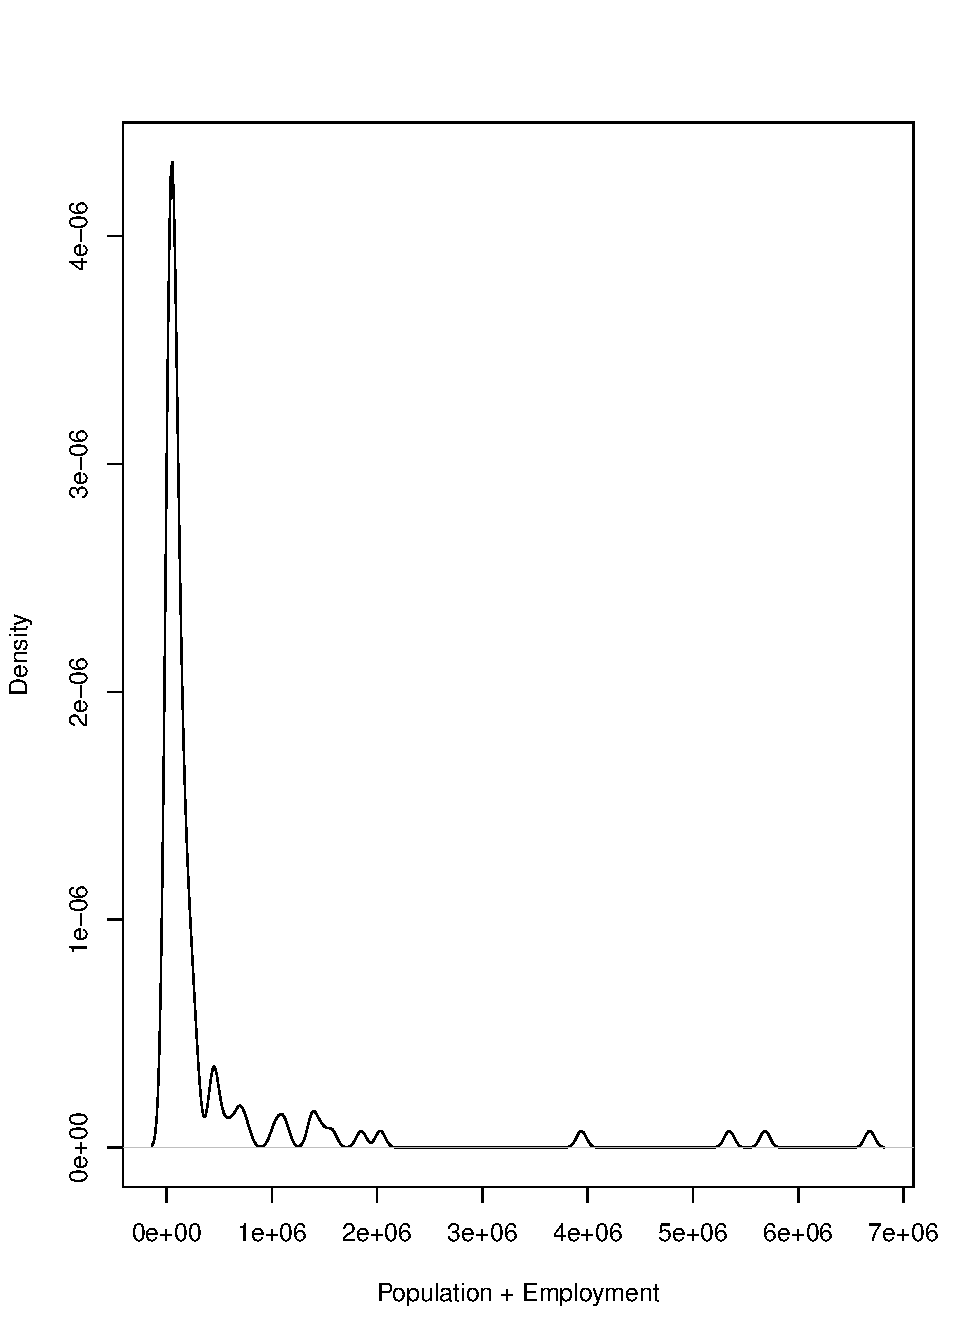
\includegraphics[height=0.6\textheight]{popEmpDensity}
\caption{Long tail and right skew of (population + employment) for each destination}
\label{fig:pop-emp-density}
\end{figure}


\begin{figure}[H]
\centering
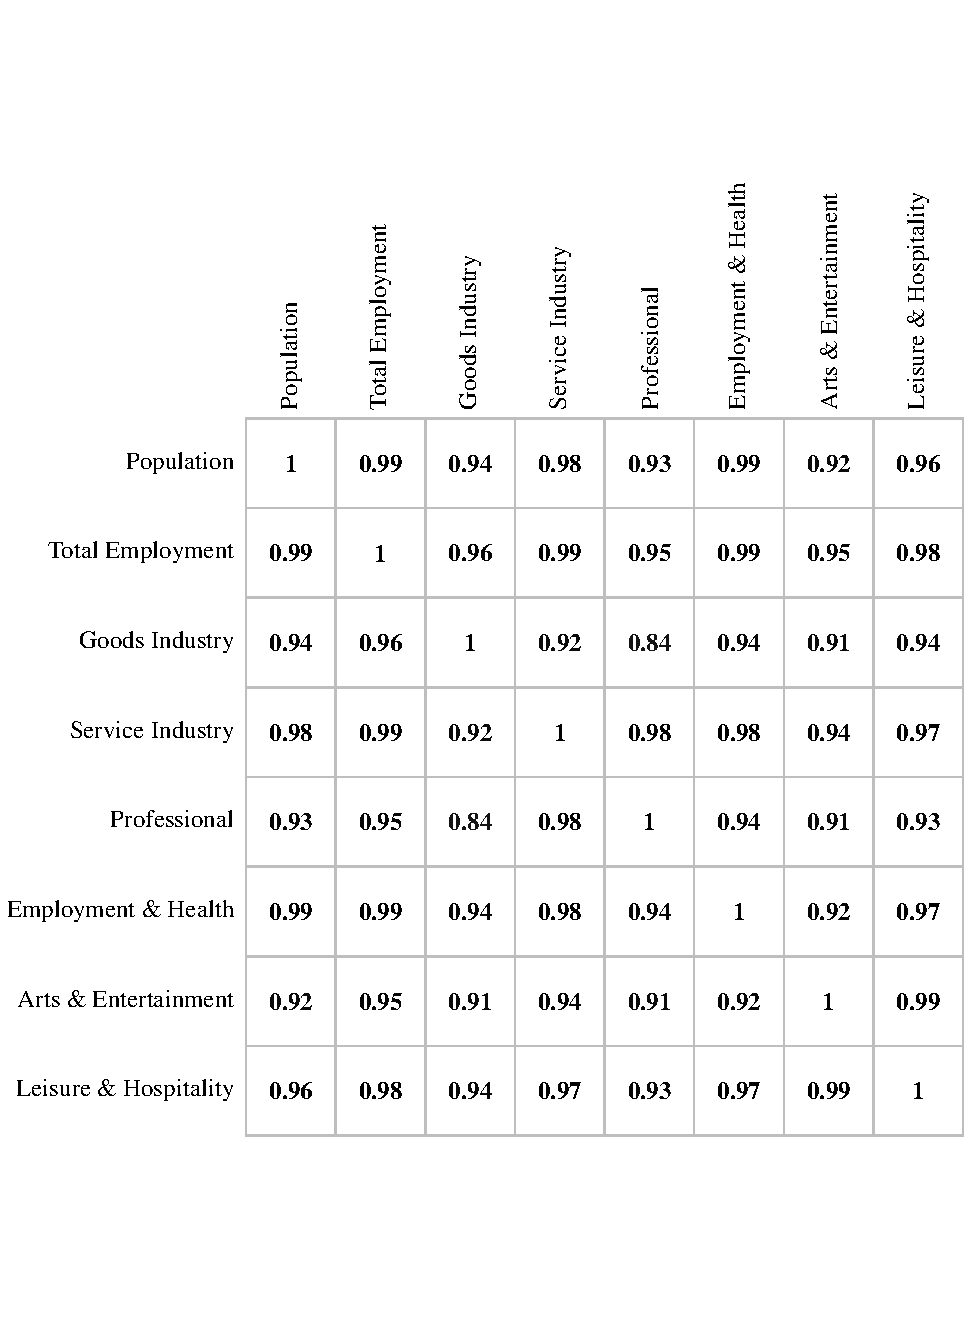
\includegraphics[width=\textwidth]{employment_correlation_plot}
\caption{High correlation between population, employment, and various employment categories across destinations}
\label{fig:pop-emp-correlation}
\end{figure}

\begin{table}[ht]
\caption{\textit{m2} Results. \\Toronto: zones 20-22, Niagara: zone 30}
\label{table:m2-error-table}
\centering
\begin{tabular}{rrrlrrrr}
  \toprule
 & Origin & Destination & Type & Predicted & Observed & Absolute Error & Max Rel. Error \\ 
  \midrule
1 & 21 & 30 & II & 877.21 & 3695.07 & 2817.86 & 3.21 \\ 
  2 & 85 & 72 & EE & 123.67 & 2407.73 & 2284.06 & 18.47 \\ 
  3 & 21 & 20 & II & 4507.84 & 2251.48 & 2256.36 & 1.00 \\ 
  4 & 21 & 22 & II & 4844.63 & 2680.21 & 2164.42 & 0.81 \\ 
  5 & 36 & 21 & II & 1346.76 & 3085.23 & 1738.46 & 1.29 \\ 
  6 & 103 & 4 & EI & 541.86 & 2061.78 & 1519.92 & 2.80 \\ 
  7 & 103 & 21 & EI & 198.15 & 1529.83 & 1331.68 & 6.72 \\ 
  8 & 21 & 53 & II & 821.51 & 2115.53 & 1294.01 & 1.58 \\ 
  9 & 64 & 64 & II & 209.47 & 1423.02 & 1213.55 & 5.79 \\ 
  10 & 21 & 54 & II & 215.05 & 1346.02 & 1130.97 & 5.26 \\ 
  11 & 20 & 30 & II & 261.47 & 1365.27 & 1103.80 & 4.22 \\ 
  12 & 22 & 30 & II & 352.63 & 1420.03 & 1067.40 & 3.03 \\ 
  13 & 30 & 30 & II & 157.40 & 1178.94 & 1021.54 & 6.49 \\ 
  14 & 21 & 52 & II & 804.06 & 1818.06 & 1014.00 & 1.26 \\ 
  15 & 21 & 4 & II & 264.90 & 1238.33 & 973.43 & 3.67 \\ 
  16 & 29 & 21 & II & 1165.79 & 2124.10 & 958.31 & 0.82 \\ 
  17 & 29 & 30 & II & 428.45 & 1353.10 & 924.65 & 2.16 \\ 
  18 & 4 & 21 & II & 403.14 & 1318.43 & 915.28 & 2.27 \\ 
  19 & 47 & 21 & II & 631.84 & 1535.96 & 904.12 & 1.43 \\ 
  20 & 4 & 85 & IE & 1660.31 & 809.08 & 851.23 & 1.05 \\ 
   \bottomrule
\end{tabular}
\end{table}

\begin{figure}[H]
\centering
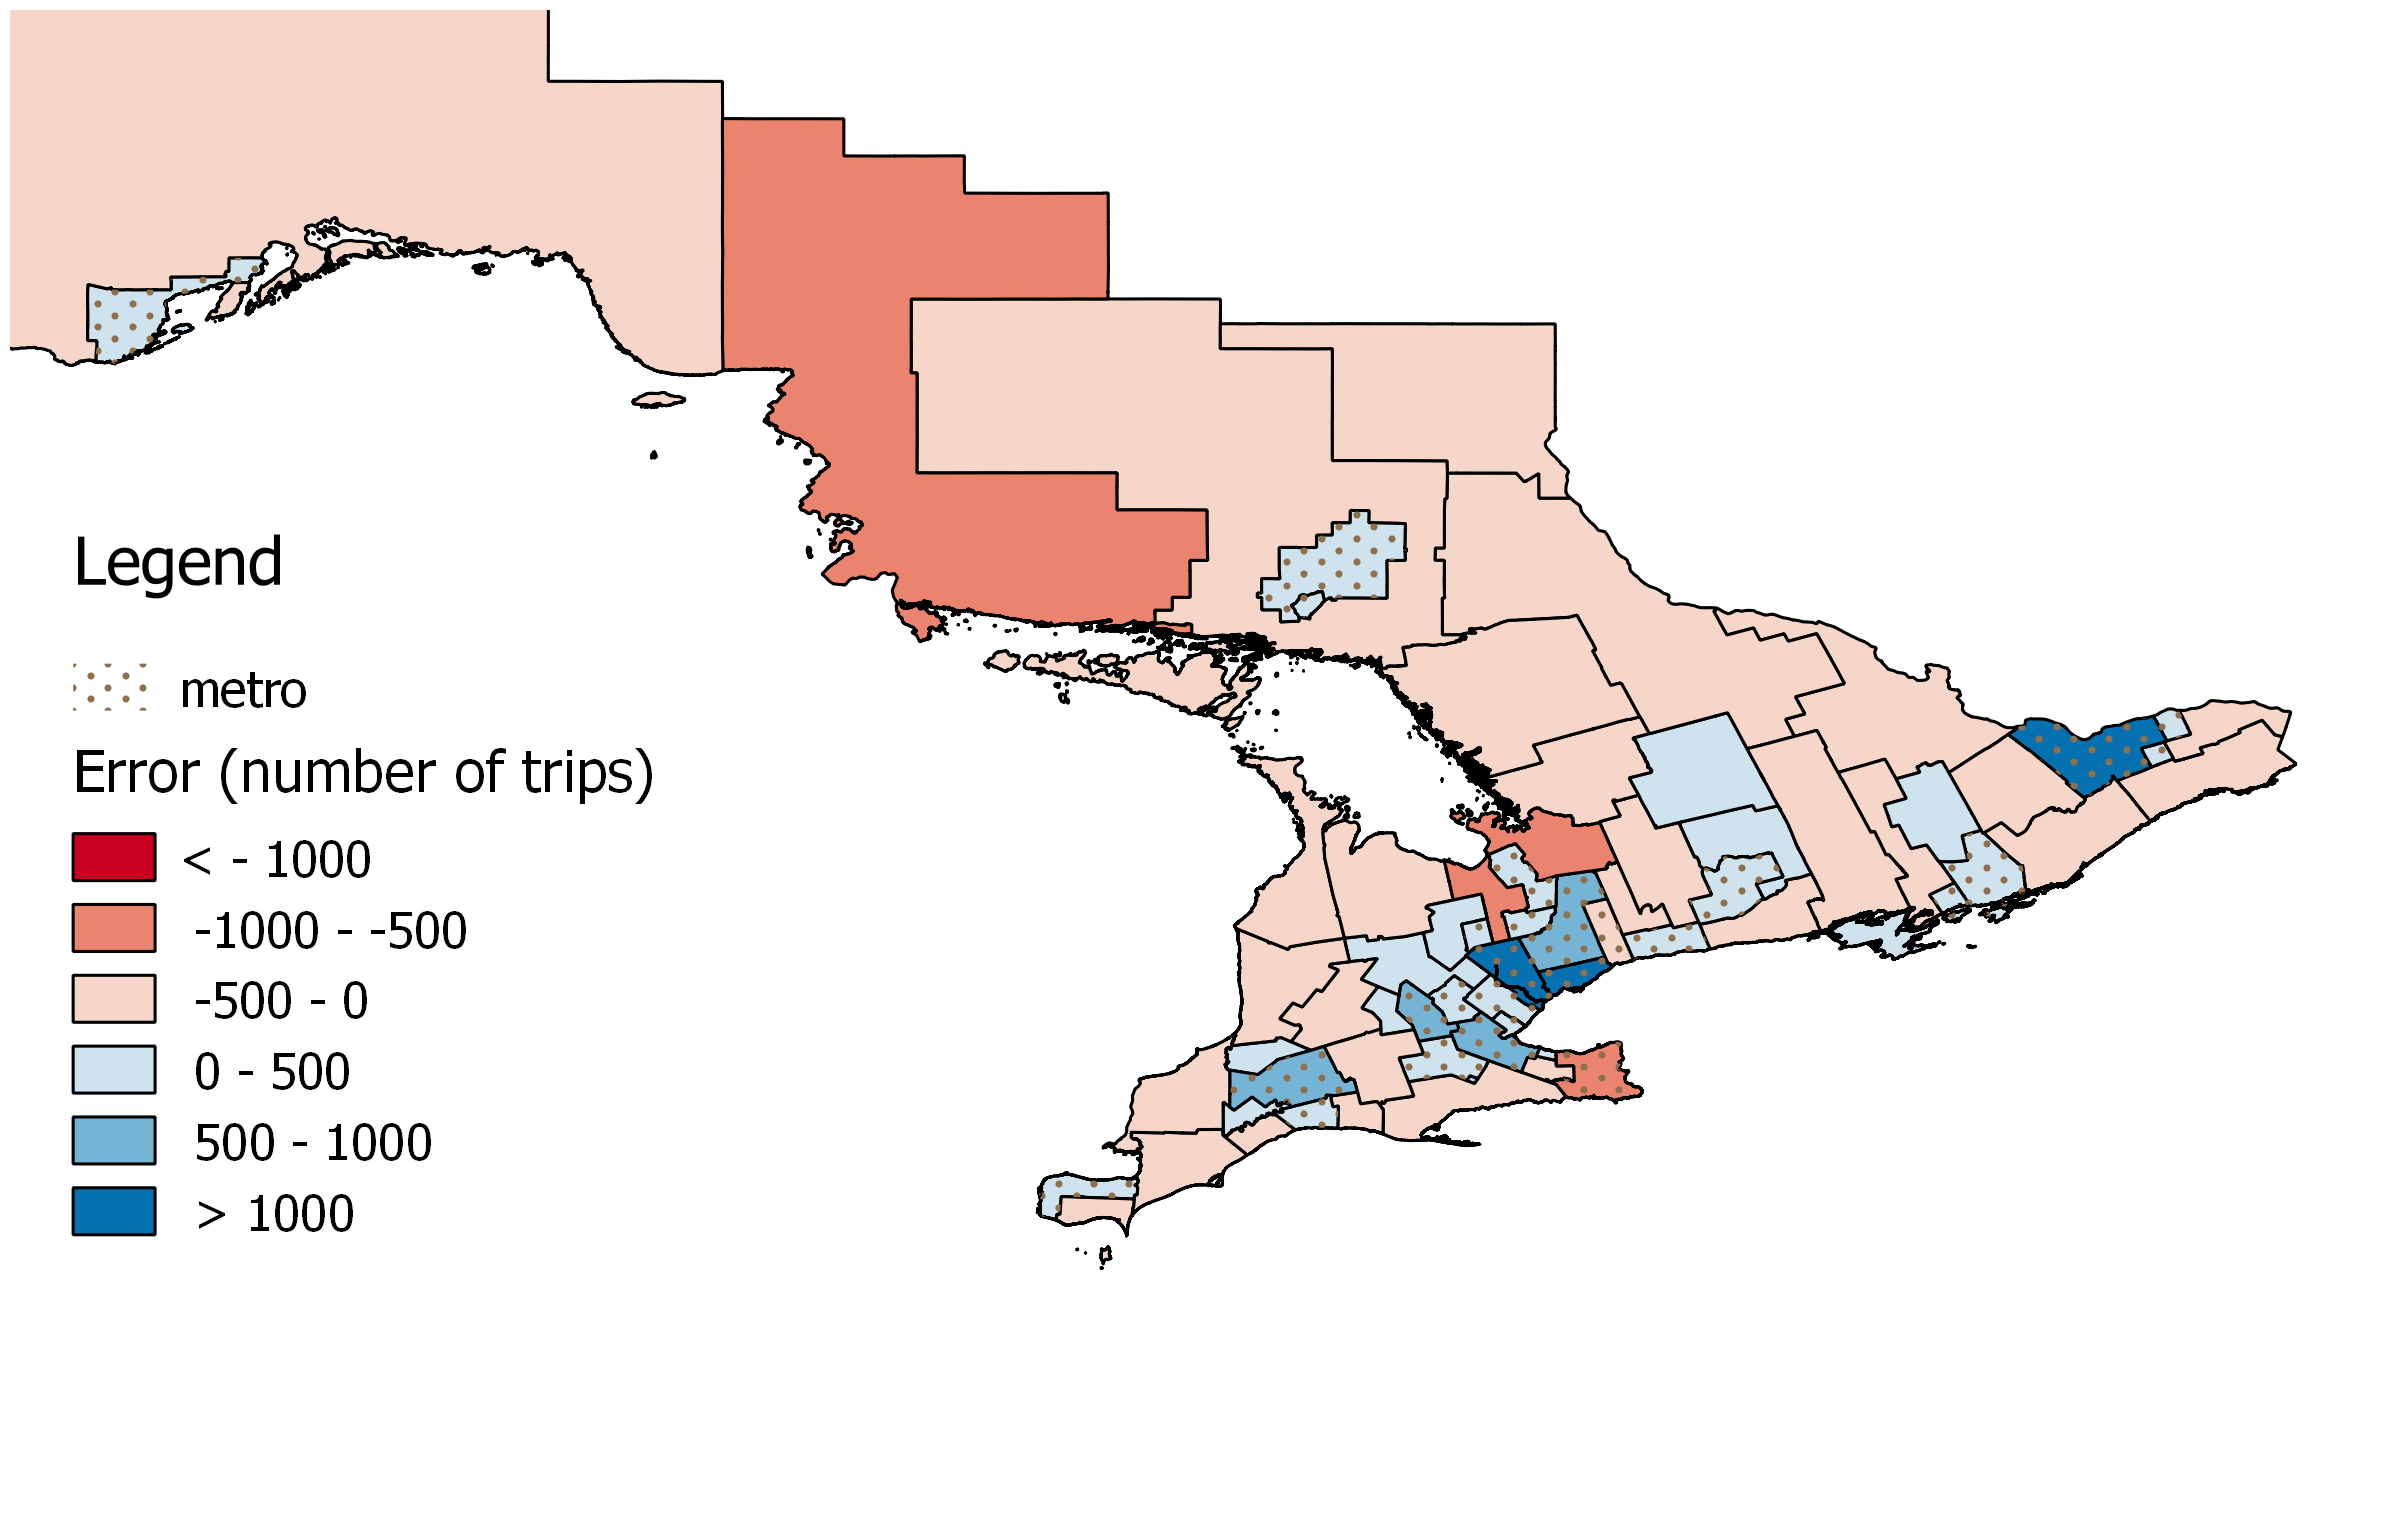
\includegraphics[width=\textwidth]{intrazonal_errors}
\caption{Intrazonal errors produced by the \textit{m2} model}
\label{fig:m2-intrazonal}
\end{figure}

\chapter{Further model results}

\begin{figure}[H]
\centering
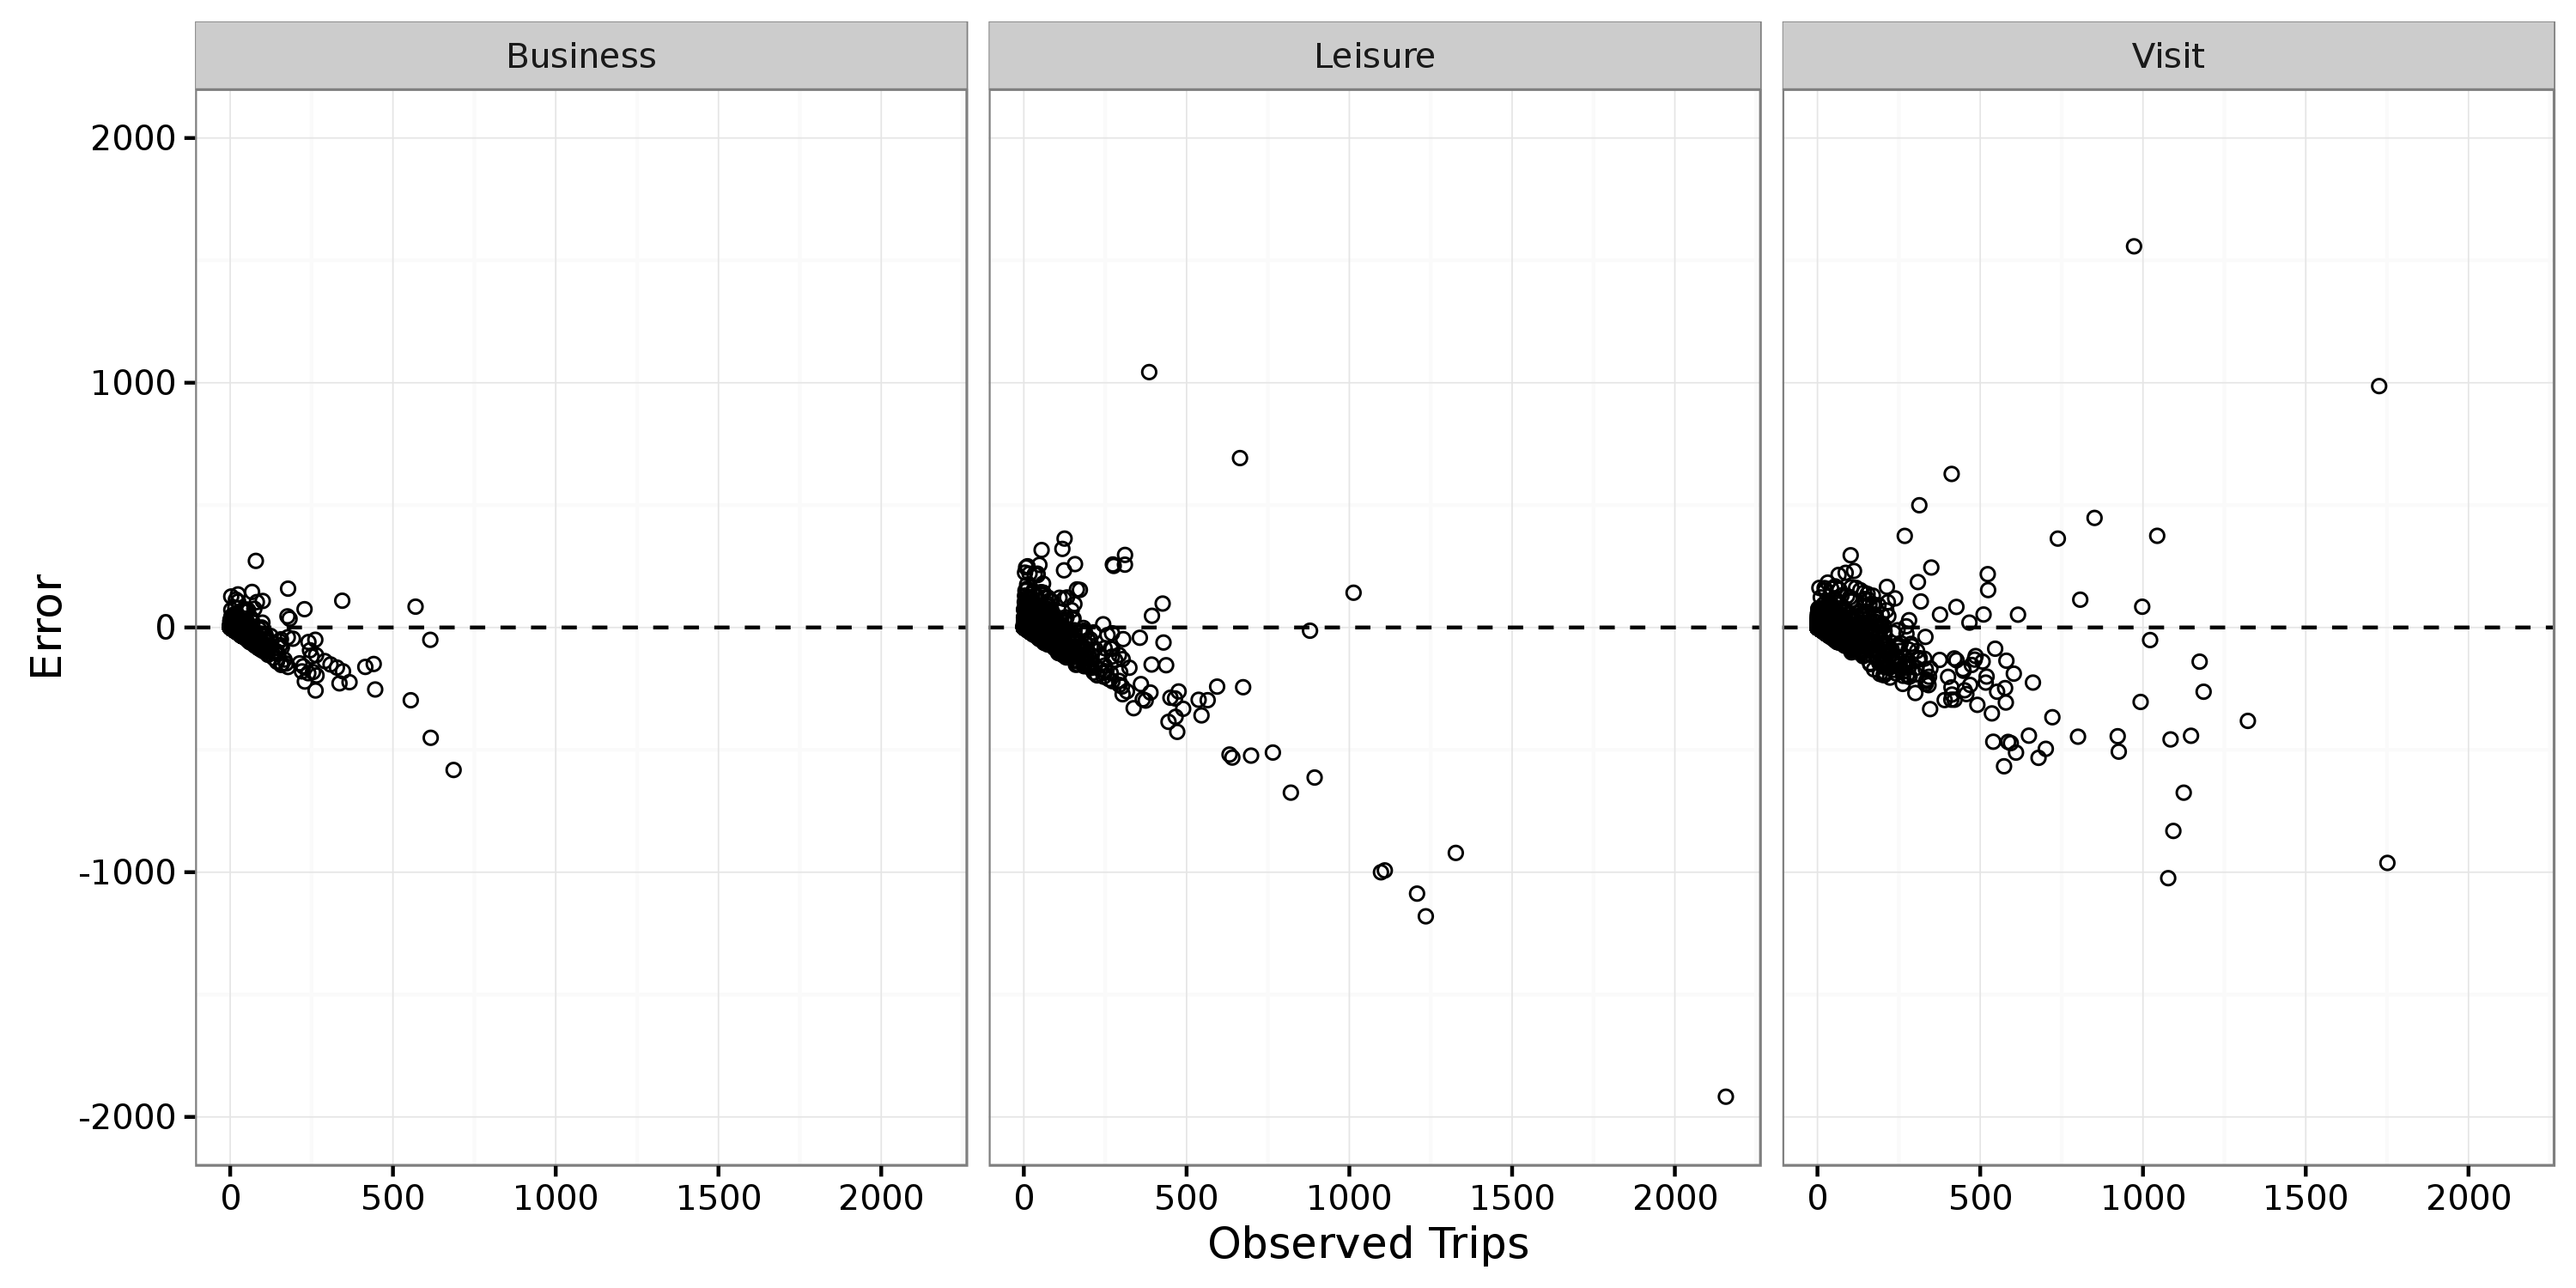
\includegraphics[width=\textwidth]{m3_residuals}
\caption{\textit{m3} model errors by observed trip count for OD pairs by trip purpose}
\label{fig:m3_residuals}
\end{figure}



